\documentclass[11pt,a4paper,ngerman]{article}
\usepackage[bottom=2.5cm,top=2.5cm]{geometry} 
\usepackage{babel}
\usepackage[utf8]{inputenc} 
\usepackage[T1]{fontenc} 
\usepackage{ae} 
\usepackage{amssymb} 
\usepackage{amsmath}
\usepackage{amsthm} 
\usepackage{graphicx}
\usepackage{fancyhdr}
\usepackage{fancyref}
\usepackage{listings}
\usepackage{xcolor}
\usepackage{paralist}
\usepackage{tabularx}
\usepackage{tikz}
\usetikzlibrary{arrows,automata}
\usepackage[pdftex, bookmarks=false, pdfstartview={FitH}, linkbordercolor=white]{hyperref}
\usepackage{fancyhdr}
\pagestyle{fancy}
\fancyhead[C]{Diskrete Mathematik}
\fancyhead[L]{Übung 6}
\fancyhead[R]{SoSe 2013}
\fancyfoot{}
\fancyfoot[L]{}
\fancyfoot[C]{\thepage \hspace{1px} of \pageref{LastPage}}
\renewcommand{\footrulewidth}{0.5pt}
\renewcommand{\headrulewidth}{0.5pt}
\setlength{\parindent}{0pt} 
\setlength{\headheight}{0pt}
\newcommand\mdoubleplus{\ensuremath{\mathbin{+\mkern-10mu+}}}
\date{}
\title{Übung 6}
\author{Max Wisniewski, Alexander Steen}
\newcommand{\argmin}{\text{argmin}}
\newcommand{\argmax}{\text{argmax}}
\newcommand{\code}[1]{\langle {#1} \rangle}
\newcommand{\Z}{\mathbb{Z}}
%%
%% Enviroments for proofs and lemmas
%%
\newtheorem{lemma}{\bfseries Claim}

\begin{document}

\lstset{language=Pascal, basicstyle=\ttfamily\fontsize{10pt}{10pt}\selectfont\upshape, commentstyle=\rmfamily\slshape, keywordstyle=\rmfamily\bfseries, breaklines=true, frame=single, xleftmargin=3mm, xrightmargin=3mm, tabsize=2, mathescape=true}

\renewcommand{\figurename}{Figure}

\maketitle
\thispagestyle{fancy}

%%%%%%%%%%%%%%%%%%%%%%%%%%%%
%% Aufgabe 1
%%%%%%%%%%%%%%%%%%%%%%%%%%%%
\subsection*{Aufgabe 1.}

Gegeben die Graphen $G_1$ und $G_2$ des Übungszettels.

\subsubsection*{(a)}
Was ist das Zirkuitsystem des graphischen Matroiden von $G_1$?\\

\textbf{Lösung:}\\

\begin{equation*}\begin{split}
    \varrho = \{ 
            & \{a,b,c\},\\
            & \{ d , e, f, g \}\\
            & \{ i , j , k , l\}\}
\end{split}\end{equation*}

\subsubsection*{(b)}
Was ist das Zirkuitsystem des cographischen Matroiden von $G_1$?\\

\textbf{Lösung:}\\

\begin{equation*}\begin{split}
    \varrho = \{ 
        & \{ a , b \}, \{ a , c \}, \{ c , b \}, \\
        & \{ g , f \}, \{ g , e \}, \{ g , d \}, \\
        & \{ f , e \}, \{ f , d \}, \{ e , d \}, \\
        & \{ i , j \}, \{ j , l \}, \{ j , k \}, \\
        & \{ i , l \}, \{ i , k \}, \{ k , l \}, \\
        & \{ h \} \}
\end{split}\end{equation*}

In jedem Kreis müssen 2 Kanten durchtrennt werden. Sobald man $h$ wegnimmt
zerfällt der Graph.

\subsubsection*{(c)}
Was ist das Basissystem des graphischen Matroiden von $G_2$?\\

\textbf{Lösung:}\\

\begin{equation*}\begin{split}
    \mathcal{B} = \{
        & \{d , a , c\}, \\
        & \{d , a , b\}, \\
        & \{d , b , c \} \}
\end{split}\end{equation*}

Die Kante $d$ muss im Baum sein und zwei Kanten des des Kreises.

\subsubsection*{(d)}
Was ist das Basissystem des cographischen Matroiden von $G_2$?\\

\textbf{Lösung:}\\

\begin{equation*}\begin{split}
    \mathcal{B} = \{
        & \{ c \},\\
        & \{ a \},\\
        & \{ b \} \}
\end{split}\end{equation*}

Wir können nur eine Kante aus dem Kreis nehmen. Danach findet man keinen aufspannenden Baum mehr.

\subsection*{Aufgabe 2.}

Geben Sie die Zirkuit- und Basissysteme sowie die Rangfunktion der folgenden Matroide an:

\subsubsection*{(a)}
Cographisches Matroid.\\

\textbf{Lösung:}\\

\begin{tabular}{rl}
    Zirkuitsystem & $\{ C \, | \, C$ Kreis in $G\}$\\
    Basisystem & Alle Menge, die aus jedem Kreis in $G$ eine Kante nehmen.\\
    Rang & $r(F) = |E| - n + 1$.
\end{tabular}\\
Der Rang ist wie angegeben, da so noch genau $n-1$ Kanten 
im Graphen sind, die genau noch einen auspannenden Baum entsprechen.

\subsubsection*{(b)}
Uniformes Matroid.\\

\textbf{Lösung:}\\

Sei $\mathcal{I}$ ein $r$ Uniformes Matroid.\\

\begin{tabular}{rl}
    Zirkuitsystem & $\varrho = \left( \begin{array}{c} M \\ r+1 \end{array}\right) $\\
    Basissystem & $\mathcal{B} = \left( \begin{array}{c} M \\ r \end{array} \right)$\\
    Rang & $r(V) = \min \{r, |V|\}$
\end{tabular}\\
Im Falle der Basis ist der Rang $r$.

\subsubsection*{(c)}
Partitionsmatroid.\\

\textbf{Lösung:}\\

Seien $M_i$ die disjunkten Mengen mit $M = \overset{k}{\underset{i=1}{\bigcup}} M_i$ und $0 \leq k_i \leq |M_i|$
ganze Zahlen.\\

\begin{tabular}{rl}
    Zirkuitsystem & $\varrho = \overset{k}{\underset{i=1}{\bigcup}} \{ M' \subset M_i \, | \, |M' \cap M_i| = k_i + 1 \} $\\
    Basissystem & $\mathcal{B} = \{ M' \subset M_1 \, | \, |M' \cap M_1| = k_1\} \times ... \times \{ M' \subset M_k \, | \, |M' \cap M_k| = k_n $\\
        &wobei hier $\times$ die paarweise Vereinigung der Mengen darstellen soll.\\
    Rang & $r(M') = \overset{k}{\underset{i=0}{\sum}} k_i$\\
\end{tabular}\\

\subsection*{Aufgabe 3.}

Sei $G = (V,E)$ ein Graph und $\mathcal{I}$ des Unabhängigkeits der stabilen Mengen in $G$.

\subsubsection*{(a)}
Stellen Sie $\mathcal{I}$ als Durchschnitt von Matroiden auf $V$ dar, d.h. 
$\mathcal{I} = \overset{k}{\underset{i=1}{\bigcap}} \mathcal{I}_i$ für
geeignet konstruierte Matroide $\mathcal{I}_i$ $i = 1, ..., k$.\\

\textbf{Lösung:}\\

Aufgabenteil b) ist allgemeiner und kann natürlich hier als Lösung verwendet werden.


\subsubsection*{(b)}
Zeigen Sie, dass sich jedes Unabhängigkeitssystem als Durchschnitt von Matroiden
darstellen lässt.\\

\textbf{Lösung:}\\

Sei $\mathcal{I} = (M,E)$ ein Unabhängigkeitssystem.
Seien $C_i$ $i=1,...,n$ die Zirkuite von $\mathcal{I}$.
Dann ist 
$\mathcal{I}_i = (M, \{F \subseteq M \, | \, C \setminus F \not= \emptyset \})$
ein Matroid.\\
\textbf{Beweis:}\\
$\emptyset \in \mathcal{I}_i$, da $C \not = \emptyset$. Daher ist $C \setminus \emptyset \not= \emptyset$\\
Falls $X$ unabhängige Menge ist und $X' \subset X$ mit $e \in X' \cap X$.
Dann ist $e \not\in C \setminus X \not= \emptyset$. So gilt $C \setminus X' \not= \emptyset$.\\

Jede Basis enthält alle Elemente
aus $M \setminus C$, da diese aufzunehmen die Bedingung an die unabhängigkeit
nicht zerstören kann. Nun enthält jede Inklusionsmaximale Menge $Z \subseteq M$
genau $|C| - 1$ Elemente von $C$. Ein Element mehr von $C$ und das Teilen
ergibt die Nullmenge. Eins weiniger und wir können es adden. Damit
hat jede Basis $|M| - 1$ Elemente. 
\mbox{}\hfill$\square$

Also sind alle $\mathcal{I}_i$ Matroide und offensichtlich ist
$\mathcal{I} = (M, \overset{n}{\underset{i=1}{\bigcap}} \mathcal{I}_i)$,
da wir in den einzelnen Matroiden alles außer den Zirkuiten von $\mathcal{I}$ 
fehlt. Damit sind nur die Zirkuite nicht im Schnitt und wir erlangen $\mathcal{I}$.
\mbox{}\hfill$\square$

\subsection*{Aufgabe 4.}
Konstruieren Sie ein Worstcase.\\

\textbf{Lösung:}\\

Wir suchen eine Gewichtsminimal Basis für stabile Mengen in eingem Graphen
$G = (V,E)$.

Sei der Graph gegeben durch das Bild \ref{disk:ueb6:wc}.

\begin{figure}[h!]
    \centering
    \frame{
    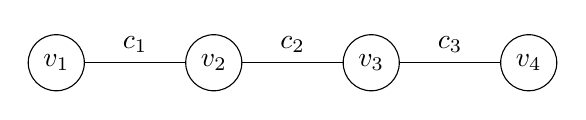
\begin{tikzpicture}
        [node distance=2cm]
        \node [circle,draw=black,name=b]{$v_2$};
        \node [circle,draw=black,name=a,left of=b] {$v_1$};
        \node [circle,draw=black,name=c,right of=b] {$v_3$};
        \node [circle,draw=black,name=d,right of=c] {$v_4$};

        \path[-] (a) edge node[above] {$c_1$} (b)
              (b) edge node[above] {$c_2$} (c)
              (c) edge node[above] {$c_3$} (d);
    \end{tikzpicture}
    }
    \caption{Worstcase für Aufgabe 4}
    \label{disk:ueb6:wc}
\end{figure}

Wenn nun $c_1 < c_2$ und $c_1 < c_3$, dann wird vom Algorithmus immer zuerst $\overline{v_1v_2}$
in die Lösung aufgenommen. Da dies keine Basis ist, wird die letzte mögliche Kante noch mitgenommen,
was hier $\overline{v_3v_4}$ ist.

Sei nun $c_2 < c_1 + c_3$ und damit die Kante $\overline{v_2v_3}$ die optimale Lösung.
Dann ist die Lösung
\begin{equation}
    d(G) = \frac{c_2}{c_1 + c_3}
\end{equation}
als der Quotient von optimaler Lösung und genommener Lösung beliebig schlecht skalierbar,
da wir $c_3$ beliebig groß wählen können ohne, dass der Algorithmus etwas anderes nehmen würde.
Mit $c_3 \rightarrow \infty$ konvergiert der Quotient gegen $0$.

\label{LastPage}

\end{document}
